\newcommand{\dropperTagResultsAucTable}{
    \begin{table}[H]
        \centering
        \begin{tabular}{|p{2,8cm}||p{2,8cm} p{2,8cm} p{2,8cm}|}
            \hline
            Dropper Tag & ALOHA & Joint Embedding & Proposed Model \\
            \hline
            AUC-ROC & 0.972$\pm$0.001 & 0.973$\pm$0.001 & \textBF{0.975$\pm$0.002} \\
            \hline
        \end{tabular}
        \caption{AUC-ROC (Area Under Curve) of the different models for the \textbf{Dropper Tag} prediction task. Results were aggregated over \textBF{3} training runs with different weight initializations and minibatch orderings. Best results are shown in \textbf{bold}.} \label{tab:dropperTag_auc}
    \end{table}
}

\newcommand{\dropperTagResultsAtFprTable}{
    \begin{center}
        \begin{longtable}[c]{|p{3,2cm}||p{1,8cm} p{1,8cm} p{1,8cm} p{1,8cm} p{1,8cm}|}
            \hline
            Dropper Tag & \multicolumn{5}{c|}{{FPR}} \\
            & $10^{-5}$ & $10^{-4}$ & $10^{-3}$ & $10^{-2}$ & $10^{-1}$ \\
            \hline
            \endfirsthead

            \caption*{\raggedright ...continued from previous page} \\
            \hline
            Dropper Tag & \multicolumn{5}{c|}{\textbf{FPR}} \\
            & $10^{-5}$ & $10^{-4}$ & $10^{-3}$ & $10^{-2}$ & $10^{-1}$ \\
            \hline
            \endhead

            \caption*{\raggedleft ...continued on next page} \\
            \endfoot

            \caption{Mean and standard deviation results (TPR, Accuracy, Recall, Precision and F1-Score) of the different models for the \textbf{Dropper Tag} prediction task at different \textbf{FPR}s (\textit{False Positive Rates}). Results were aggregated over \textBF{3} training runs with different weight initializations and minibatch orderings. Best results are shown in \textbf{bold}. Under \textbf{TPR} results are also presented the percentage reduction in mean detection error and in ROC curve standard deviation introduced by the \textit{Proposed Model} with respect to both \textit{ALOHA} model and \textit{Joint Embedding}.} \label{tab:dropperTag_results_at_fpr} \\
            \endlastfoot

            \multicolumn{6}{|c|}{\textbf{TPR}} \\
            \hline
            ALOHA & 0.045$\pm$0.007 & 0.068$\pm$0.021 & 0.121$\pm$0.063 & 0.672$\pm$0.026 & \textBF{0.921$\pm$0.011} \\
            Joint Embedding & \textBF{0.118$\pm$0.078} & 0.159$\pm$0.132 & 0.179$\pm$0.131 & \textBF{0.730$\pm$0.011} & 0.910$\pm$0.015 \\
            Proposed Model & 0.089$\pm$0.035 & \textBF{0.174$\pm$0.041} & \textBF{0.265$\pm$0.057} & 0.729$\pm$0.035 & 0.916$\pm$0.006 \\
            \hline
            Error Reduction wrt \newline ALOHA & 4.6\% & 11.4\% & 16.4\% & 17.4\% & -6.3\% \\
            Error Reduction wrt \newline Joint Embedding & -3.3\% & 1.8\% & 10.5\% & -0.4\% & 6.7\% \\
            \hline
            Std Reduction wrt \newline ALOHA & -400.0\% & -95.2\% & 9.5\% & -34.6\% & 45.5\% \\
            Std Reduction wrt \newline Joint Embedding & 55.1\% & 68.9\% & 56.5\% & -218.2\% & 60.0\% \\
            \hline
            \multicolumn{6}{|c|}{\textbf{Accuracy}} \\
            \hline
            ALOHA & 0.878$\pm$0.001 & 0.881$\pm$0.003 & 0.887$\pm$0.008 & 0.949$\pm$0.003 & \textBF{0.903$\pm$0.001} \\
            Joint Embedding & \textBF{0.887$\pm$0.010} & 0.893$\pm$0.017 & 0.894$\pm$0.017 & \textBF{0.957$\pm$0.001} & 0.901$\pm$0.002 \\
            Proposed Model & 0.884$\pm$0.004 & \textBF{0.894$\pm$0.005} & \textBF{0.905$\pm$0.007} & 0.957$\pm$0.004 & 0.902$\pm$0.001 \\
            \hline
            \multicolumn{6}{|c|}{\textbf{Recall}} \\
            \hline
            ALOHA & 0.045$\pm$0.007 & 0.068$\pm$0.021 & 0.121$\pm$0.063 & 0.672$\pm$0.026 & \textBF{0.921$\pm$0.011} \\
            Joint Embedding & \textBF{0.118$\pm$0.078} & 0.159$\pm$0.132 & 0.179$\pm$0.131 & \textBF{0.730$\pm$0.011} & 0.910$\pm$0.015 \\
            Proposed Model & 0.089$\pm$0.035 & \textBF{0.173$\pm$0.041} & \textBF{0.265$\pm$0.057} & 0.729$\pm$0.035 & 0.916$\pm$0.006 \\
            \hline
            \multicolumn{6}{|c|}{\textbf{Precision}} \\
            \hline
            ALOHA & \textBF{0.999$\pm$0.000} & 0.989$\pm$0.004 & 0.931$\pm$0.035 & 0.908$\pm$0.003 & \textBF{0.574$\pm$0.003} \\
            Joint Embedding & 0.999$\pm$0.001 & 0.992$\pm$0.005 & 0.944$\pm$0.029 & \textBF{0.914$\pm$0.001} & 0.571$\pm$0.004 \\
            Proposed Model & \textBF{0.999$\pm$0.000} & \textBF{0.996$\pm$0.001} & \textBF{0.974$\pm$0.006} & 0.914$\pm$0.004 & 0.573$\pm$0.002 \\
            \hline
            \multicolumn{6}{|c|}{\textbf{F1 Score}} \\
            \hline
            ALOHA & 0.086$\pm$0.013 & 0.127$\pm$0.038 & 0.210$\pm$0.098 & 0.772$\pm$0.019 & \textBF{0.707$\pm$0.005} \\
            Joint Embedding & \textBF{0.203$\pm$0.121} & 0.253$\pm$0.186 & 0.282$\pm$0.177 & \textBF{0.812$\pm$0.007} & 0.702$\pm$0.007 \\
            Proposed Model & 0.162$\pm$0.059 & \textBF{0.293$\pm$0.061} & \textBF{0.414$\pm$0.072} & 0.811$\pm$0.023 & 0.705$\pm$0.003 \\
            \hline
        \end{longtable}
    \end{center}
}

\newcommand{\dropperTagResultsSummaryTable}{
    \begin{table}[H]
        \centering
        \begin{tabular}{|p{3,2cm}||p{1,8cm} p{1,8cm} p{1,8cm} p{1,8cm} p{1,8cm}|}
            \hline
            \multicolumn{6}{|c|}{Dropper Tag (at FPR $=1\%$)} \\
            \hline
            Model & TPR & Accuracy & Precision & Recall & F1 score \\
            \hline
            ALOHA & 0.672$\pm$0.026 & 0.949$\pm$0.003 & 0.908$\pm$0.003 & 0.672$\pm$0.026 & 0.772$\pm$0.019 \\
            Joint Embedding & \textBF{0.730$\pm$0.011} & \textBF{0.957$\pm$0.001} & \textBF{0.914$\pm$0.001} & \textBF{0.730$\pm$0.011} & \textBF{0.812$\pm$0.007} \\
            Proposed Model & 0.729$\pm$0.035 & 0.957$\pm$0.004 & 0.914$\pm$0.004 & 0.729$\pm$0.035 & 0.811$\pm$0.023 \\
            \hline
        \end{tabular}
        \caption{Summary of the mean and standard deviation results of the different models for the \textbf{Dropper Tag} prediction task at \textbf{FPR} $=1\%$. Results were aggregated over \textBF{3} training runs with different weight initializations and minibatch orderings. Best results are shown in \textbf{bold}.} \label{tab:dropperTag_result_summary}
    \end{table}
}

\newcommand{\dropperTagRocAloha}{
    \begin{figure}[H]
        \vspace*{-0.5cm}
        \centering
        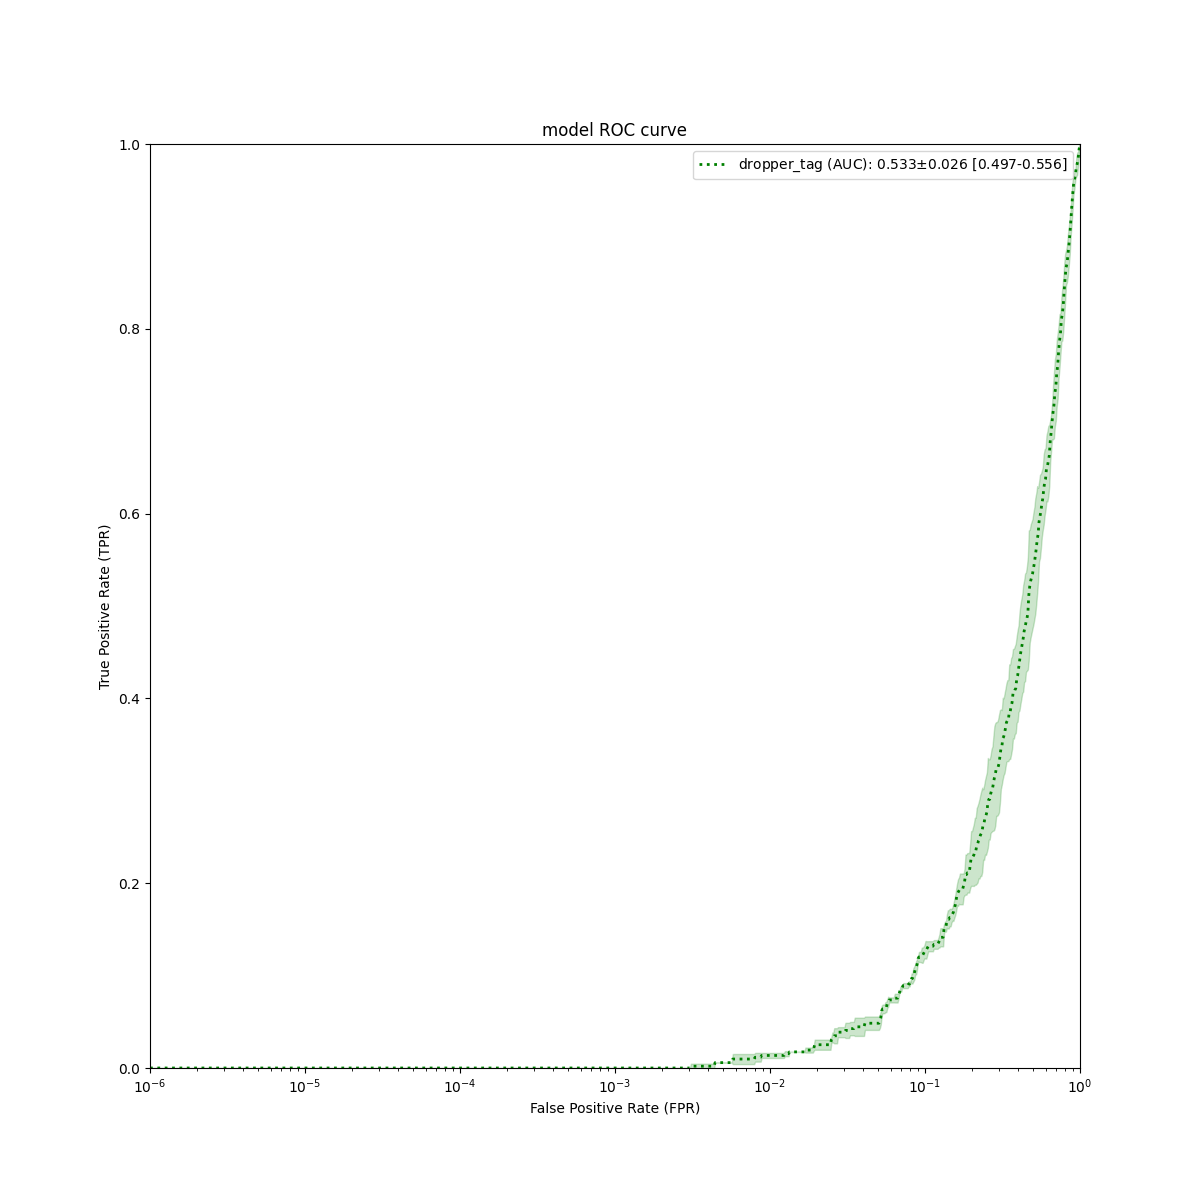
\includegraphics[width=0.6\textwidth]{./results/dropper_tag_roc_aloha.png}
        \vspace*{-0.2cm}
        \caption{ROC curve and AUC statistics of \textBF{ALOHA} model for the \textbf{Dropper Tag}. The line represents the \textit{mean} TPR at a given FPR, while the shaded region represents the \textit{standard deviation}. Statistics were computed over \textBF{3} training runs, each with random parameter initialization.}
        \label{fig:dropperTagRocAloha}
    \end{figure}
}

\newcommand{\dropperTagRocJointEmbedding}{
    \begin{figure}[H]
        \vspace*{-0.5cm}
        \centering
        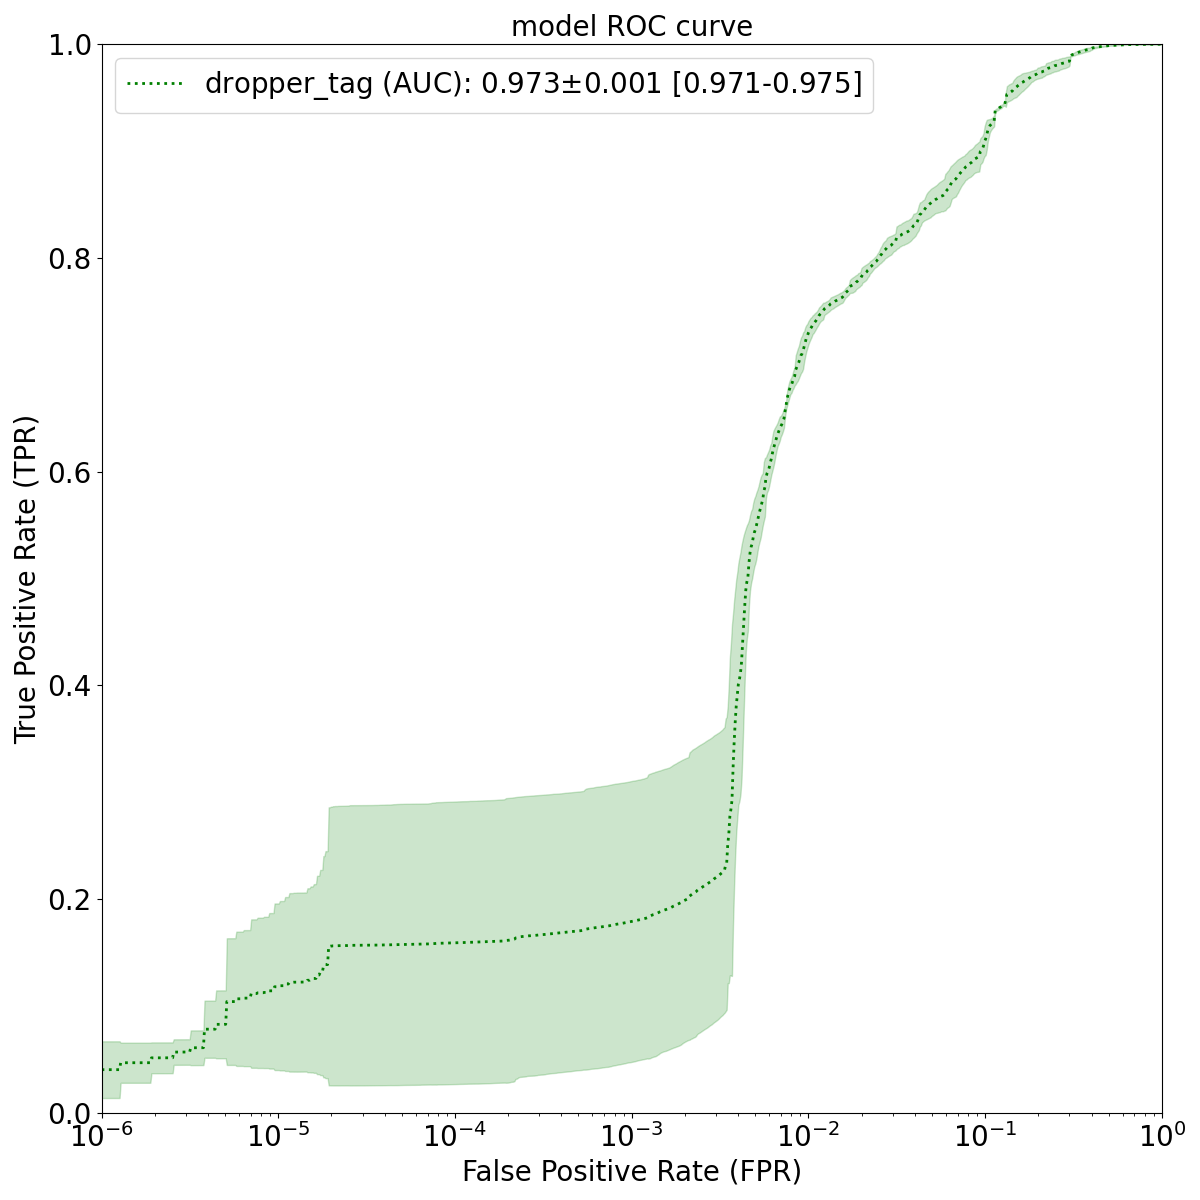
\includegraphics[width=0.6\textwidth]{./results/dropper_tag_roc_jointEmbedding.png}
        \vspace*{-0.2cm}
        \caption{ROC curve and AUC statistics of \textBF{Joint Embedding} model for the \textbf{Dropper Tag}. The line represents the \textit{mean} TPR at a given FPR, while the shaded region represents the \textit{standard deviation}. Statistics were computed over \textBF{3} training runs, each with random parameter initialization.}
        \label{fig:dropperTagRocJointEmbedding}
    \end{figure}
}

\newcommand{\dropperTagRocProposedMethod}{
    \begin{figure}[H]
        \vspace*{-0.5cm}
        \centering
        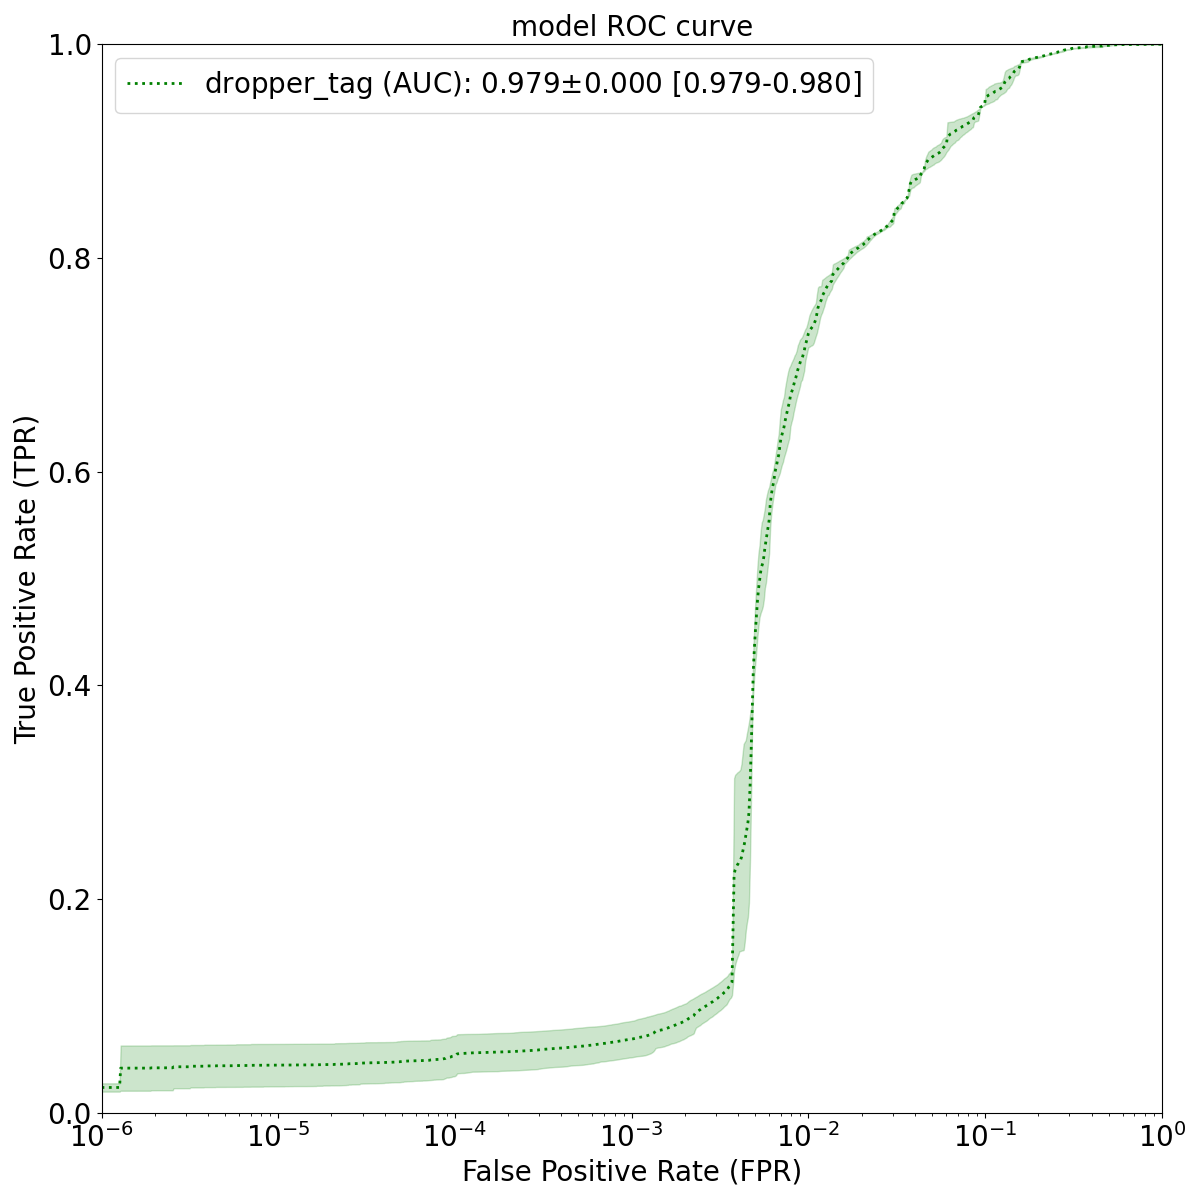
\includegraphics[width=0.6\textwidth]{./results/dropper_tag_roc_proposedModel.png}
        \vspace*{-0.2cm}
        \caption{ROC curve and AUC statistics of \textBF{Proposed Model} for the \textbf{Dropper Tag}. The line represents the \textit{mean} TPR at a given FPR, while the shaded region represents the \textit{standard deviation}. Statistics were computed over \textBF{3} training runs, each with random parameter initialization.}
        \label{fig:dropperTagRocProposedModel}
    \end{figure}
}
